%\documentclass[fleqn,compress,utf8,aspectratio=169,t]{beamer}
\documentclass[fleqn,compress,utf8,aspectratio=169,t,handout]{beamer}
% use LMU theme
\usetheme{LMU}

% This setups a lot of recommended settings and packages you usually need
% anyway. So let me take care for you and your document stays clear.

% Examples: Tables, Graphics, Listings, Hyperref...
%
% Prevent slide breaks in the middle of a paragraph
\widowpenalties 1 10000
\raggedbottom

\makeatletter
\@ifundefined{KOMAClassName}{% if non-KOMA class
  \IfFileExists{parskip.sty}{%
    \RequirePackage{parskip}
  }{% else
    \setlength{\parindent}{0pt}
    \setlength{\parskip}{6pt plus 2pt minus 1pt}}
}{% if KOMA class
  \KOMAoptions{parskip=half}}
\makeatother

\IfFileExists{xurl.sty}{\usepackage{xurl}}{} % add URL line breaks if available
\IfFileExists{bookmark.sty}{\usepackage{bookmark}}{\usepackage{hyperref}}
\urlstyle{same} % disable monospaced font for URLs

\usepackage{listings}
\lstset{defaultdialect=[5.3]Lua}
\lstset{defaultdialect=[x86masm]Assembler}
\usepackage{longtable,booktabs}
\usepackage{caption}
% Make caption package work with longtable
\makeatletter
\def\fnum@table{\tablename~\thetable}
\makeatother
\usepackage{graphicx}
\makeatletter
\def\maxwidth{\ifdim\Gin@nat@width>\linewidth\linewidth\else\Gin@nat@width\fi}
\def\maxheight{\ifdim\Gin@nat@height>\textheight\textheight\else\Gin@nat@height\fi}
\makeatother
% Scale images if necessary, so that they will not overflow the page
% margins by default, and it is still possible to overwrite the defaults
% using explicit options in \includegraphics[width, height, ...]{}
\setkeys{Gin}{width=\maxwidth,height=\maxheight,keepaspectratio}
% Set default figure placement to htbp
\makeatletter
\def\fps@figure{htbp}
\makeatother
\usepackage[normalem]{ulem}
% Avoid problems with \sout in headers with hyperref
\pdfstringdefDisableCommands{\renewcommand{\sout}{}}
\setlength{\emergencystretch}{3em} % prevent overfull lines
%Tightlist Command
\providecommand{\tightlist}{%
  \setlength{\itemsep}{0pt}\setlength{\parskip}{0pt}}



%%%%%%%%%%%%%%%%%%%%%%%%%%%%%%%%%%%%%%%%%%%%%%%%%%%%%%%%%%%%%%%%%%%%%%%%%%%%%%%%
%%                                Citation styles                             %%
%%%%%%%%%%%%%%%%%%%%%%%%%%%%%%%%%%%%%%%%%%%%%%%%%%%%%%%%%%%%%%%%%%%%%%%%%%%%%%%%

%%% VERSION 1
%if you want to cite in the text
%\usepackage[style=ext-authoryear]{biblatex}
%\DeclareOuterCiteDelims{parencite}{\bibopenbracket}{\bibclosebracket}
%and use the command \parencite

%%% VERSION 2
%if you want to cite using a footnote	
\usepackage[style=authortitle]{biblatex}
\renewcommand{\thempfootnote}{\arabic{mpfootnote}}
%use the command \footcite
% change \vspace{NUMex}} to place your footnote a bit higher
\addtobeamertemplate{footnote}{}{\vspace{5ex}}

\addbibresource{lmu-example.bib}

\setbeamersize{text margin left=13pt,text margin right=13pt}





%%%%%%%%%%%%%%%%%%%%%%%%%%%%%%%%%%%%%%%%%%%%%%%%%%%%%%%%%%%%%%%%%%%%%%%%%%%%%%%%
%%                                 Own packages                               %%
%%%%%%%%%%%%%%%%%%%%%%%%%%%%%%%%%%%%%%%%%%%%%%%%%%%%%%%%%%%%%%%%%%%%%%%%%%%%%%%%

\usepackage[T1]{fontenc}
\usepackage{lmodern}
%\usepackage{blindtext}
%\usepackage{lmodern}
\usepackage{amsmath}
\usepackage{csquotes}


\usepackage{amssymb}
\usepackage{amsthm}
%\usepackage{chngcntr}   %für \counterwithout
\usepackage{pict2e} 		%für "picture"-Umgebung(s. 1.6.7)
\usepackage{graphicx}
\usepackage[ngerman,english]{babel}     %ngerman: Latex-Default, english: Default for this document!
\usepackage{fancyhdr}
\usepackage{color}
%\usepackage{cases}	%f\"ur numcases
\usepackage{mathtools}   % loads »amsmath«
\usepackage{algorithm,algorithmicx}
%\usepackage[]{algorithm2e}
\usepackage[noend]{algpseudocode}
% \usepackage{empheq}
%% \usepackage{a4wide}
\usepackage{datetime}
\usepackage{ulem}
\usepackage{fancybox}
\usepackage{tikz}
\usetikzlibrary{arrows.meta}
\usepackage{subcaption}
%\usepackage[babel=true]{csquotes}
\usepackage{microtype}  %Verbessert das Schriftbild erheblich, weniger Probleme mit overfullboxes, von Karlson
%\usepackage{booktabs} 
%\usepackage{subfigure}

\usepackage{enumitem}
\usepackage{nicefrac}

%%%%%%%%%%%%%%%%%%%%%%%%%%%%%%%%%%%%%%%%%%%%%%%%%%%%%%%%%%%%%%%%%%%%%%%%%%%%%%%%
%%                                 Own commands                             %%
%%%%%%%%%%%%%%%%%%%%%%%%%%%%%%%%%%%%%%%%%%%%%%%%%%%%%%%%%%%%%%%%%%%%%%%%%%%%%%%%


\newcommand{\R}{{\mathbb{R}}}
%\newcommand{\C}{{\mathbb{C}}}
\newcommand{\N}{{\mathbb{N}}}
\newcommand{\Z}{{\mathbb{Z}}}
\newcommand{\Q}{{\mathbb{Q}}}
\newcommand{\E}{{\mathbb{E}}}
\renewcommand{\P}{{\mathbb{P}}}
\newcommand{\F}{{\mathcal{F}}}
\newcommand{\Borel}[1]{{\mathcal{B}( #1 )}}
\newcommand{\NV}[2]{{\mathcal{N}( #1 , #2 )}}		%Normalverteilt
\renewcommand{\Re}[1]{\text{Re($#1$)}}
\renewcommand{\Im}[1]{\text{Im($#1$)}}
\newcommand{\vect}[2]{\begin{pmatrix} #1 \\ #2\end{pmatrix}}
\newcommand{\norm}[1]{\left| \left| #1 \right| \right|}
\newcommand{\IP}[2]{{\left\langle #1, #2 \right\rangle  }}
\newcommand{\ra}{{\rightarrow}}
\newcommand{\Ra}{{\Rightarrow}}
\newcommand{\Lra}{{\Leftrightarrow}}
\newcommand{\DefLra}{{: \Leftrightarrow}}
\newcommand{\ind}{{{\perp\!\!\!\perp}}}		%independent
\newcommand{\eps}{{\varepsilon}}
\newcommand{\floor}[1]{{\lfloor #1 \rfloor}}
\newcommand{\sgn}{{\textrm{sgn}}}
\newcommand{\ol}[1]{\overline{#1}}
\newcommand{\blue}[1]{{{\color{blue}#1}}} 
\newcommand{\red}[1]{{{\color{red}#1}}} 
\newcommand{\ul}[1]{\underline{#1}}
\newcommand{\Qabbr}[3]{{Q_{[#1,#2,#3]}}}
\newcommand{\Qexpand}[3]{{\begin{pmatrix} - & #1 & #3 \\ & - & #2 \\ & & -\end{pmatrix}}}
\renewcommand{\qed}{\text{ } \text{ }\hfill\ensuremath{\blacksquare}}
\newcommand{\qedwhite}{\hfill \hfill\ensuremath{\Box}}
\def\Xint#1{\mathchoice
	{\XXint\displaystyle\textstyle{#1}}%
	{\XXint\textstyle\scriptstyle{#1}}%
	{\XXint\scriptstyle\scriptscriptstyle{#1}}%
	{\XXint\scriptscriptstyle\scriptscriptstyle{#1}}%
	\!\int}
\def\XXint#1#2#3{{\setbox0=\hbox{$#1{#2#3}{\int}$}
		\vcenter{\hbox{$#2#3$}}\kern-.5\wd0}}
\def\ddashint{\Xint=}
\def\dashint{\Xint-}

%\usepackage{appendixnumberbeamer}

%%%%%%%%%%%%%%%%%%%%%%%%%%%%%%%%%%%%%%%%%%%%%%%%%%%%%%%%%%%%%%%%%%%%%%%%%%%%%%%%
%%                                 Customizations                             %%
%%%%%%%%%%%%%%%%%%%%%%%%%%%%%%%%%%%%%%%%%%%%%%%%%%%%%%%%%%%%%%%%%%%%%%%%%%%%%%%%

% If you want no navigation uncomment this
%\beamertemplatenavigationsymbolsempty

% setup listings
\lstset{
  basicstyle=\ttfamily\color{black},
  showstringspaces=false
}

\lstdefinestyle{highlight}{
  keywordstyle=\color{red},
  commentstyle=\color{lmu@darkgray}
}

\lstdefinestyle{basetex}{
language={[LaTeX]Tex},
basicstyle=\color{black!40},
keywordstyle=\color{red!40},
commentstyle=\color{lmu@darkgray!40},
moredelim=**[il][\only<+>{\color{black}\lstset{style=highlight}}]{@}
}

\lstdefinestyle{basec}{
language=C,
basicstyle=\color{black!40},
keywordstyle=\color{red!40},
commentstyle=\color{green!40},
moredelim=**[il][\only<+>{\color{black}\lstset{style=highlight}}]{@}
}

\setlist[itemize,1]{label={\small{$\blacksquare$}}}
\setlist[itemize,2]{label={\small{$\bullet$}}}
\setlist[itemize,3]{label={$-$}}
\setlist[itemize,4]{label={$-$}}


%%%%%%%%%%%%%%%%%%%%%%%%%%%%%%%%%%%%%%%%%%%%%%%%%%%%%%%%%%%%%%%%%%%%%%%%%%%%%%%%
%%                                  Title Page Data                           %%
%%%%%%%%%%%%%%%%%%%%%%%%%%%%%%%%%%%%%%%%%%%%%%%%%%%%%%%%%%%%%%%%%
\newcommand{\addauthor}[3]{
	\parbox[c]{0.26\textwidth}{
		{\bfseries #1} \\
		{\scriptsize{#2}}\\
		{\scriptsize{#3}}
	}}
% helper command to add multiple authors
\newcommand{\newauthor}[3]{
\parbox[c]{0.26\textwidth}{
{\bfseries #1} \\
{\scriptsize{#2}}\\
{\scriptsize{#3}}
}
%{#1}
}



% add additional authors
\institute[LMU]{%
\addauthor{Lorenz}{Lorenz.Gartmeier@campus.lmu.de}{LMU Munich} \hspace{0.35cm}
\addauthor{Anatol Maier}{anatol.maier@neuraforge.de}{supervisor at Neuraforge AI Solutions GmbH}}




\date[\today]{\today}

\title{Reliable Attribution of GAN
and Diffusion-based Image Generators}
%\title{short}
%\subtitle{Paper ID: 11132}

\hypersetup{
  pdftitle={Reliable Attribution of GAN and Diffusion-based Image Generators},
  pdfauthor={Lorenz Gartmeier},
  hidelinks}
\setbeamercolor{frametitle}{fg=lmu@green}

%%%%%%%%%%%%%%%%%%%%%%%%%%%%%%%%%%%%%%%%%%%%%%%%%%%%%%%%%%%%%%%%%%%%%%%%%%%%%%%%
%%                                  Document                                  %%
%%%%%%%%%%%%%%%%%%%%%%%%%%%%%%%%%%%%%%%%%%%%%%%%%%%%%%%%%%%%%%%%%%%%%%%%%%%%%%%%

\begin{document}


\begin{frame}
  \titlepage
\end{frame}

%%%%%%%%%%%%%%%%%%%%%%%%%%%%%%%%%%% Overview %%%%%%%%%%%%%%%%%%%%%%%%%%%%%%%%%%%




\section{Introduction}

\begin{frame}
	\begin{figure}
		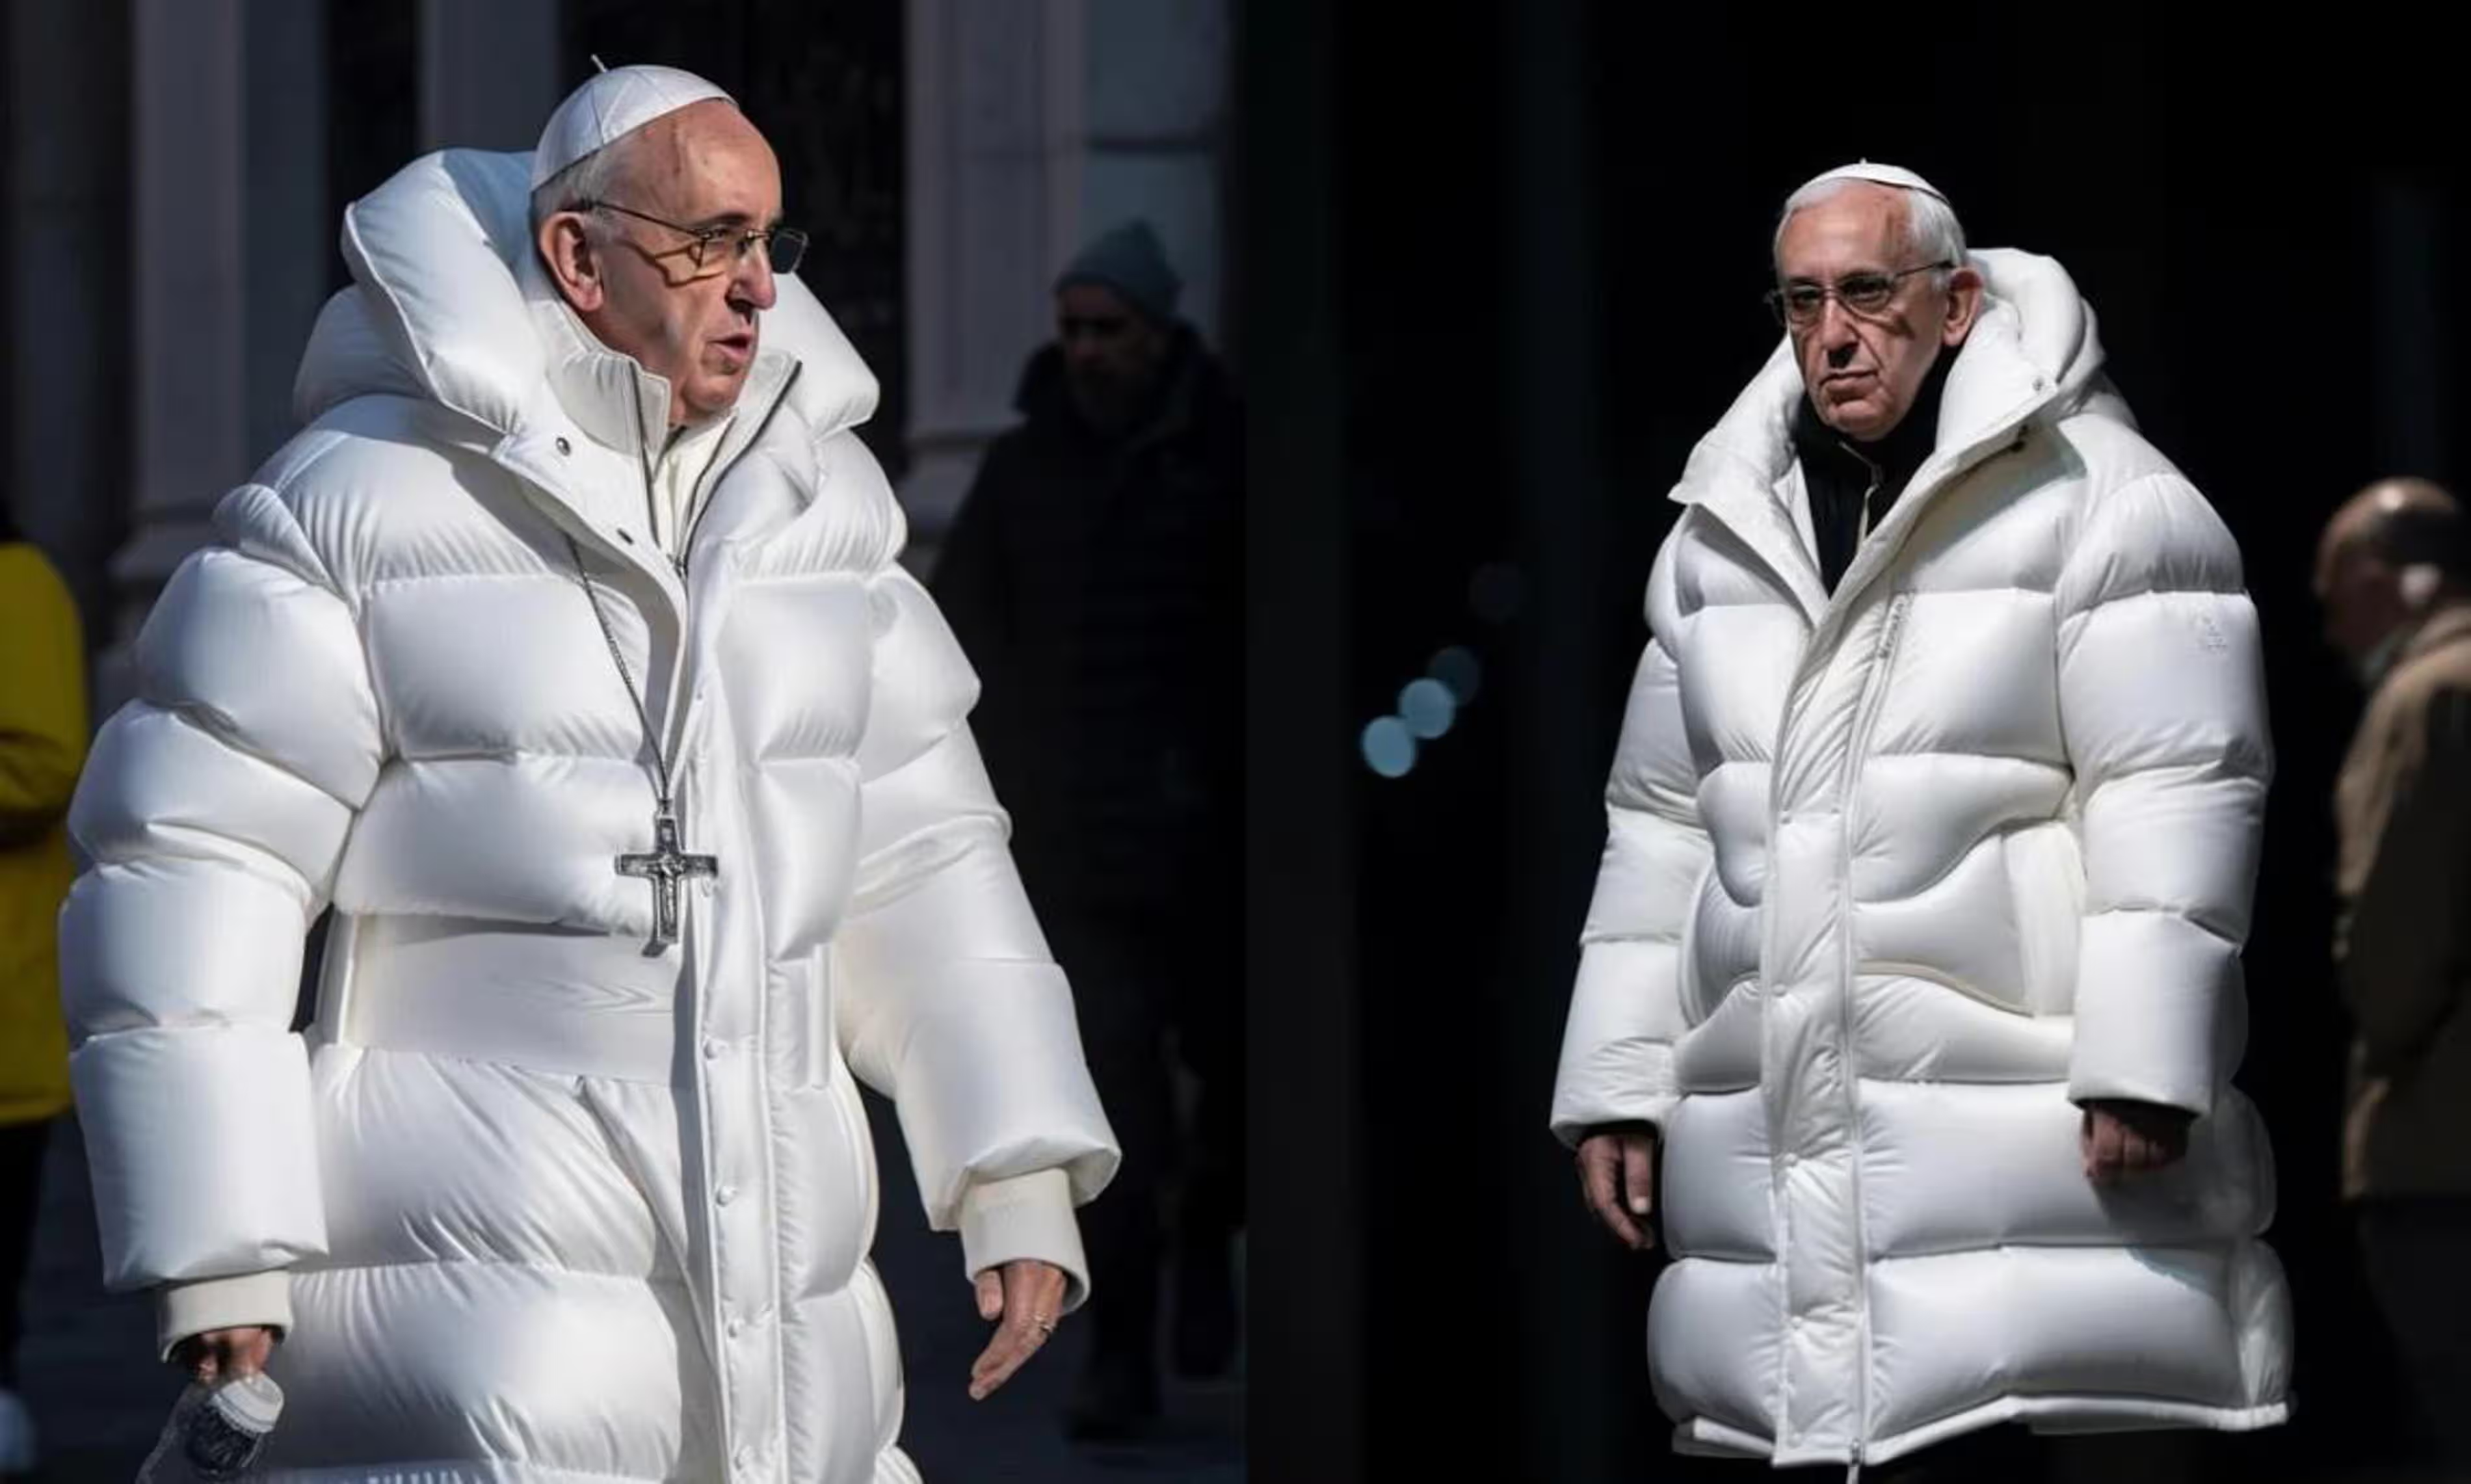
\includegraphics[width = 0.7 \textwidth]{figs/pope-in-coat.png}
		\text{\footnotesize source: https://www.theguardian.com/commentisfree/2023/mar/27/pope-coat-ai-image-baby-boomers}
	\end{figure}
\end{frame}


\begin{frame}
	\begin{figure}
		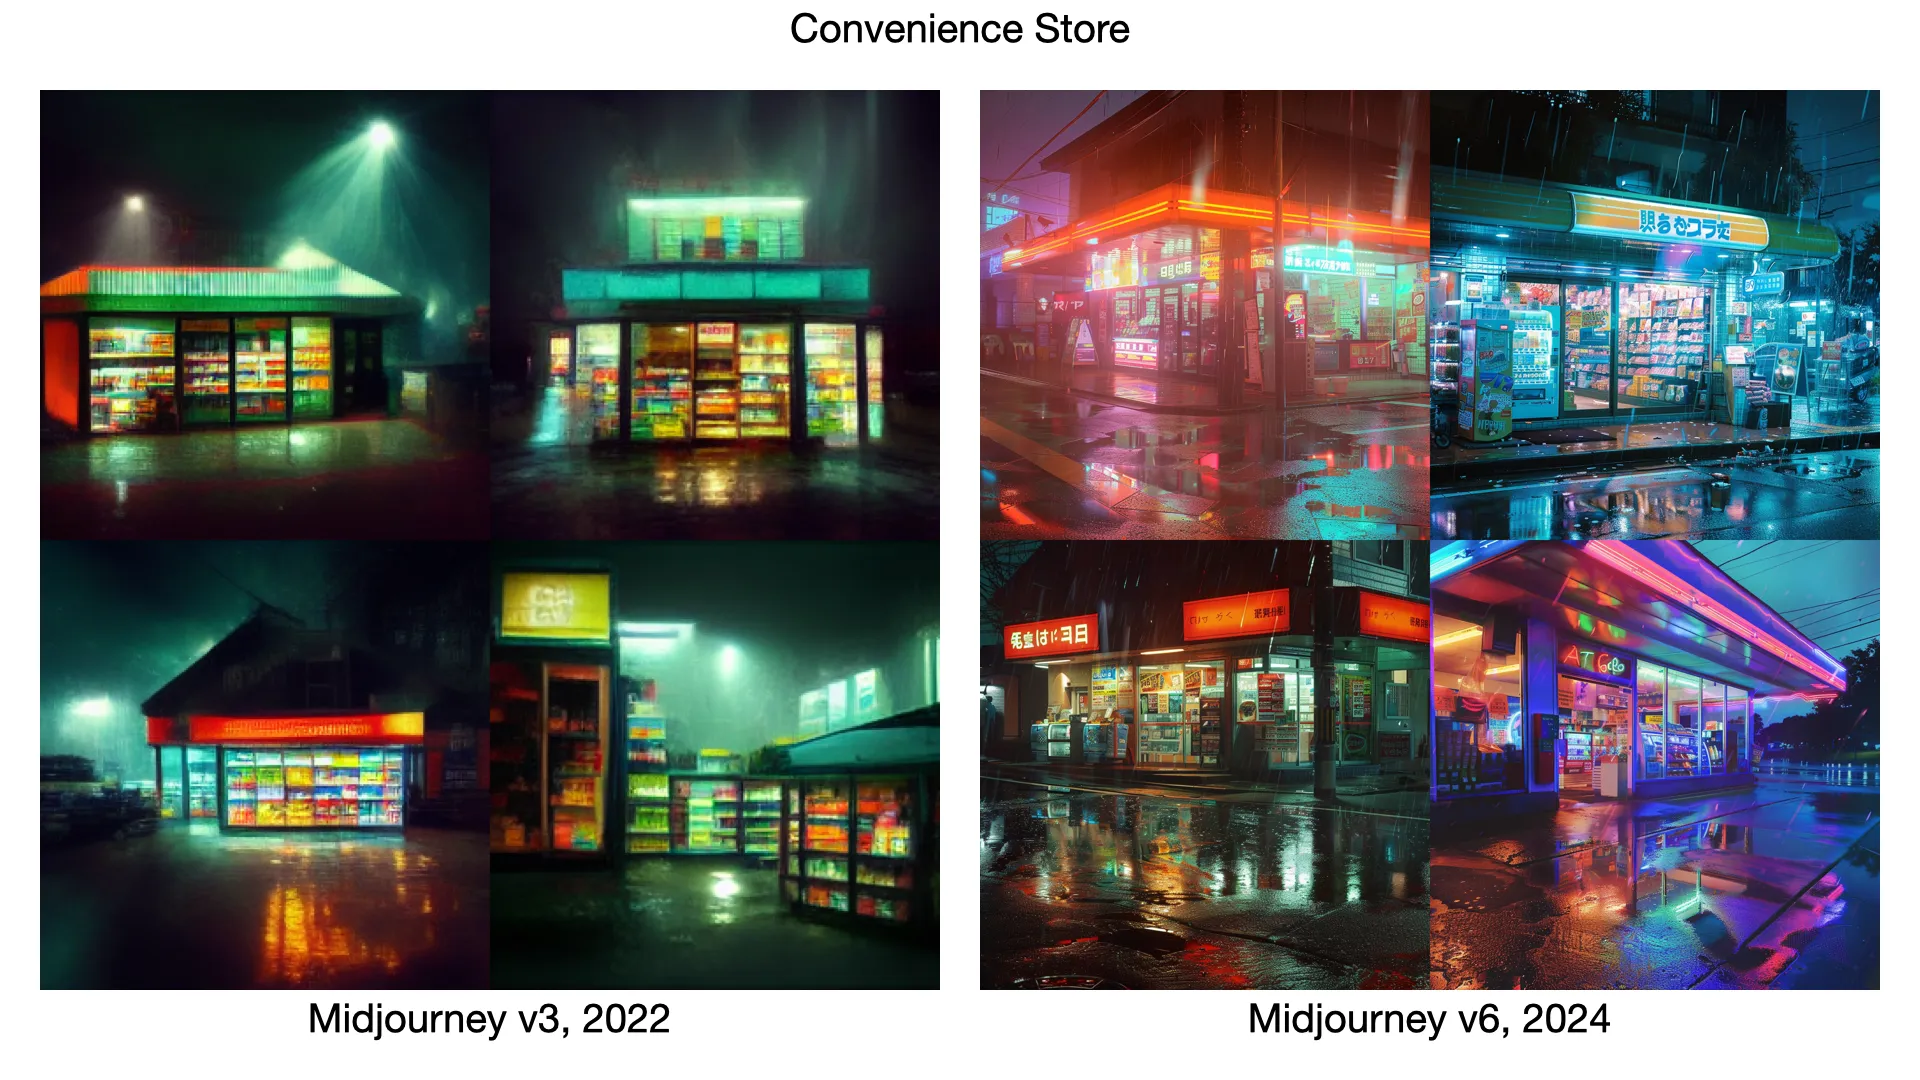
\includegraphics[width = 0.8 \textwidth]{figs/old-vs-new-generation.png}
		\text{\footnotesize source: https://medium.com/@junehao/comparing-ai-generated-images-two-years-apart}
	\end{figure}
\end{frame}

\begin{frame}
	Attribute images to source models, so that
\begin{itemize}
    \item image can be identified as fake
    \item companies can be pointed at the misuse of their product by users
    \item companies can be hold responsible 
    \item images from unknown sources don't get falsely attributed 
\end{itemize}
by using a Bayesian Deep Learning approach

\end{frame}

\section{Background}

\begin{frame}
	\begin{figure}
		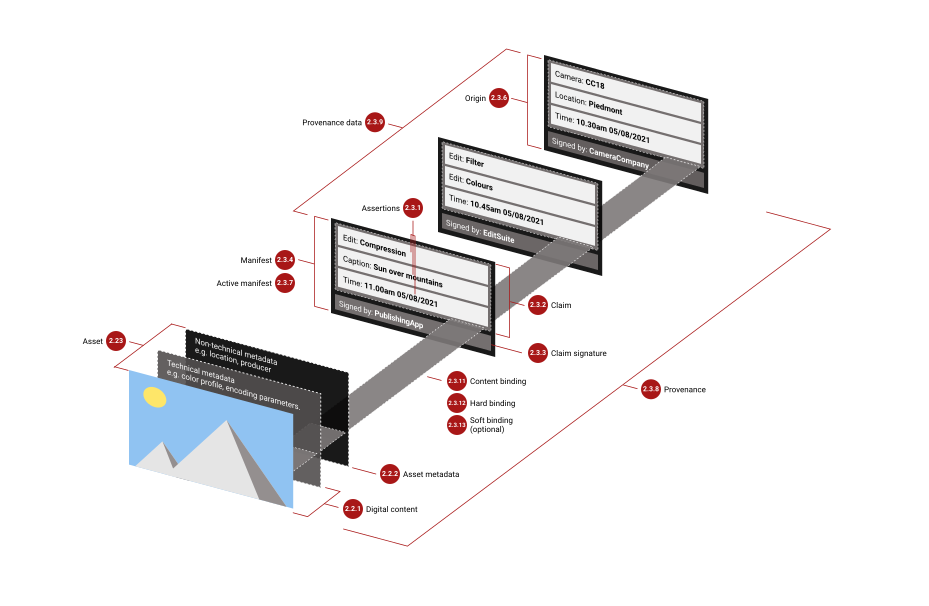
\includegraphics[width = 0.7 \textwidth]{figs/C2PA.png}
		\text{\footnotesize source: https://c2pa.org/specifications/specifications/2.1/specs/C2PA\_Specification.html}
	\end{figure}
\end{frame}

\begin{frame}
	\begin{figure}
		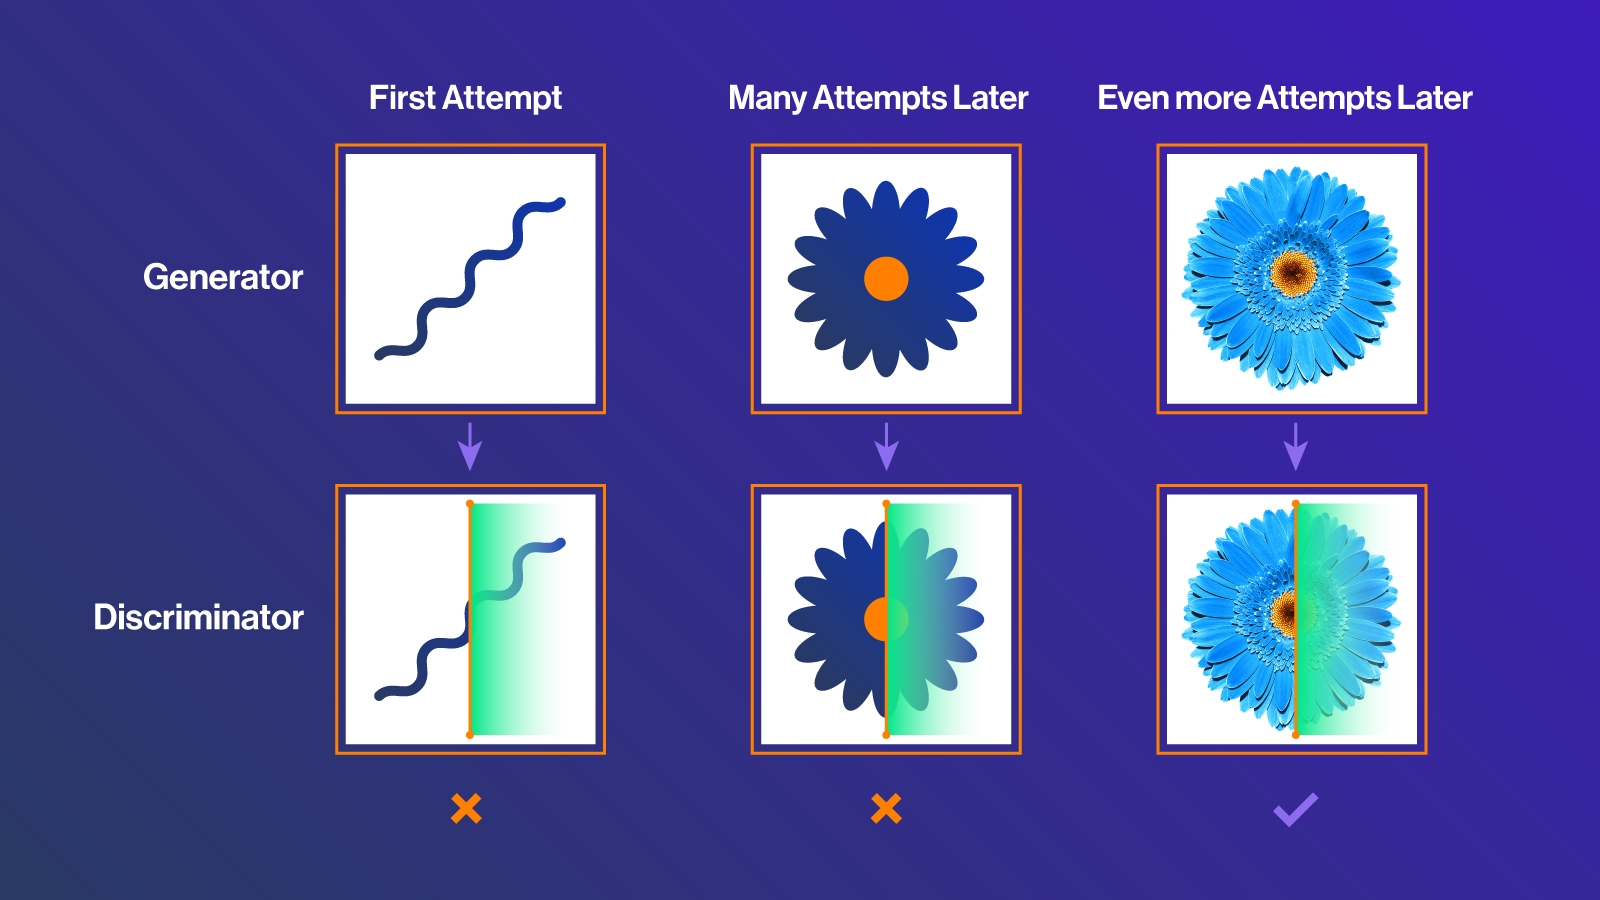
\includegraphics[width = 0.8 \textwidth]{figs/GAN-Architecture.jpg}
		\text{\footnotesize source: https://www.sabrepc.com/blog/Deep-Learning-and-AI/gans-vs-diffusion-models}
	\end{figure}
\end{frame}

\begin{frame}
	\begin{figure}
		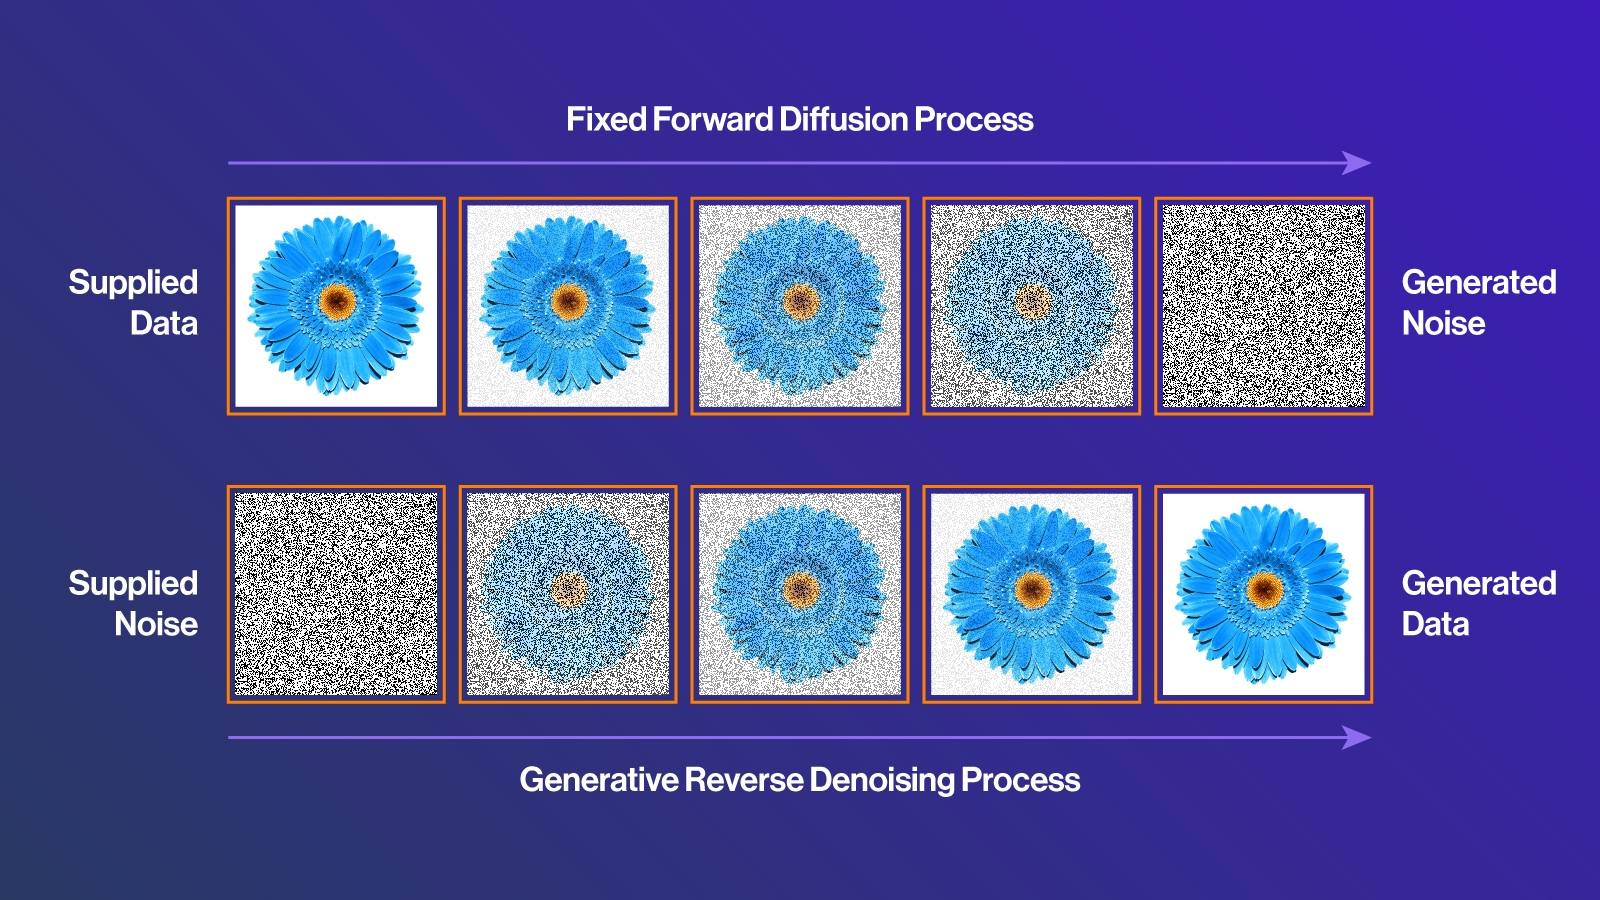
\includegraphics[width = 0.8 \textwidth]{figs/Diffusion-Architecture.jpg}
		\text{\footnotesize source: https://www.sabrepc.com/blog/Deep-Learning-and-AI/gans-vs-diffusion-models}
	\end{figure}
\end{frame}

\begin{frame}
	\begin{figure}
		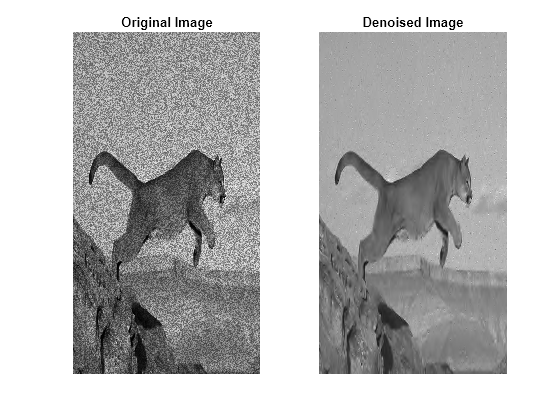
\includegraphics[width = 0.6 \textwidth]{figs/noisy-vs-denoised.png}
		\text{\footnotesize source: https://www.mathworks.com/help/wavelet/ug/wavelet-denoising.html}
	\end{figure}
\end{frame}

\begin{frame}
	\begin{figure}[h]
    \centering
    \begin{minipage}{0.45\textwidth}
      
\includegraphics[width = 0.8 \textwidth]{figs/ProGAN_Kitchen_F002.jpg}
      \caption{fingerprint estimate with 2 residuals}
    \end{minipage}
    \hfill
    \pause
		\begin{minipage}{0.45\textwidth}
      
\includegraphics[width = 0.8 \textwidth]{figs/ProGAN_Kitchen_F008.jpg}
      \caption{fingerprint estimate with 8 residuals}
    \end{minipage}
	\end{figure}
  \text{\footnotesize source: Marra et al, "Do GANs leave artificial fingerprints?", 2018}
\end{frame}

\begin{frame}
	\begin{figure}[h]
    \centering
    \begin{minipage}{0.45\textwidth}
      
\includegraphics[width = 0.8 \textwidth]{figs/ProGAN_Kitchen_F032.jpg}
      \caption{fingerprint estimate with 32 residuals}
    \end{minipage}
    \hfill
    \pause
		\begin{minipage}{0.45\textwidth}
      
\includegraphics[width = 0.8 \textwidth]{figs/ProGAN_Kitchen_F128.jpg}
      \caption{fingerprint estimate with 128 residuals}
    \end{minipage}
	\end{figure}
  \text{\footnotesize       \space source: Marra et al, "Do GANs leave artificial fingerprints?", 2018}
\end{frame}

\begin{frame}
	\begin{figure}[h]
    \centering
    \begin{minipage}{0.45\textwidth}
      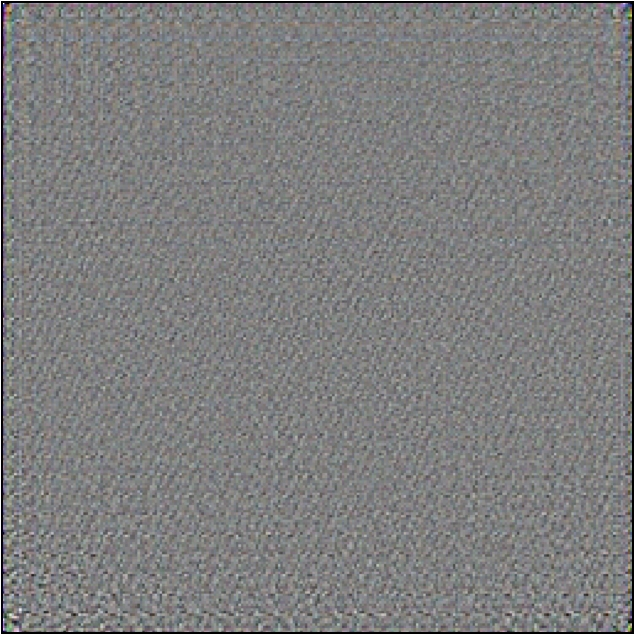
\includegraphics[width = 0.8 \textwidth]{figs/ProGAN_Kitchen_F512.jpg}
      \caption{fingerprint estimate with 512 residuals}
    \end{minipage}
    \hfill
    \pause
		\begin{minipage}{0.45\textwidth}
      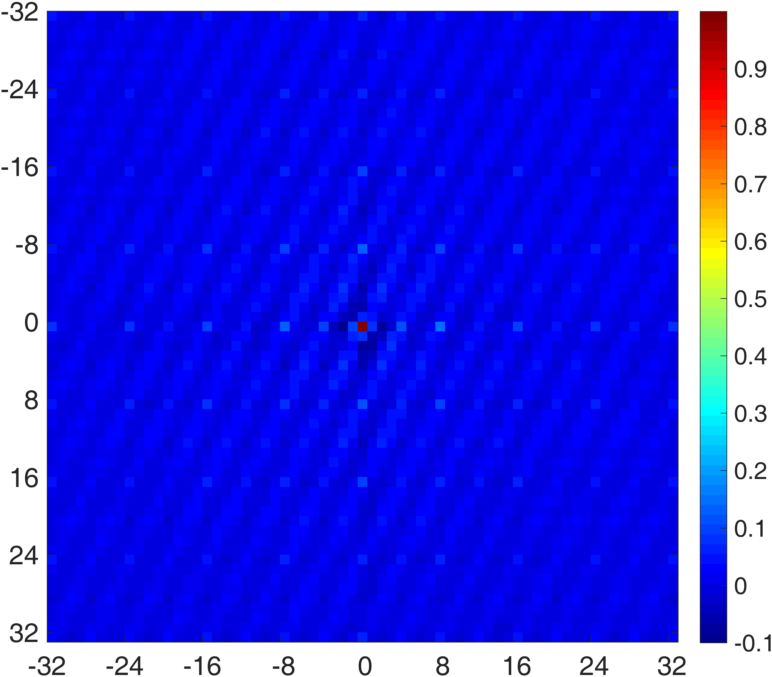
\includegraphics[width = 0.9 \textwidth]{figs/ProGAN_Kitchen_F512_autocorrelation.png}
      \caption{frequency domain}
    \end{minipage}
	\end{figure}
  \text{\footnotesize source: Marra et al, "Do GANs leave artificial fingerprints?", 2018}
\end{frame}

\begin{frame}
	\begin{figure}[h]
    \centering
    \begin{minipage}{0.3\textwidth}
      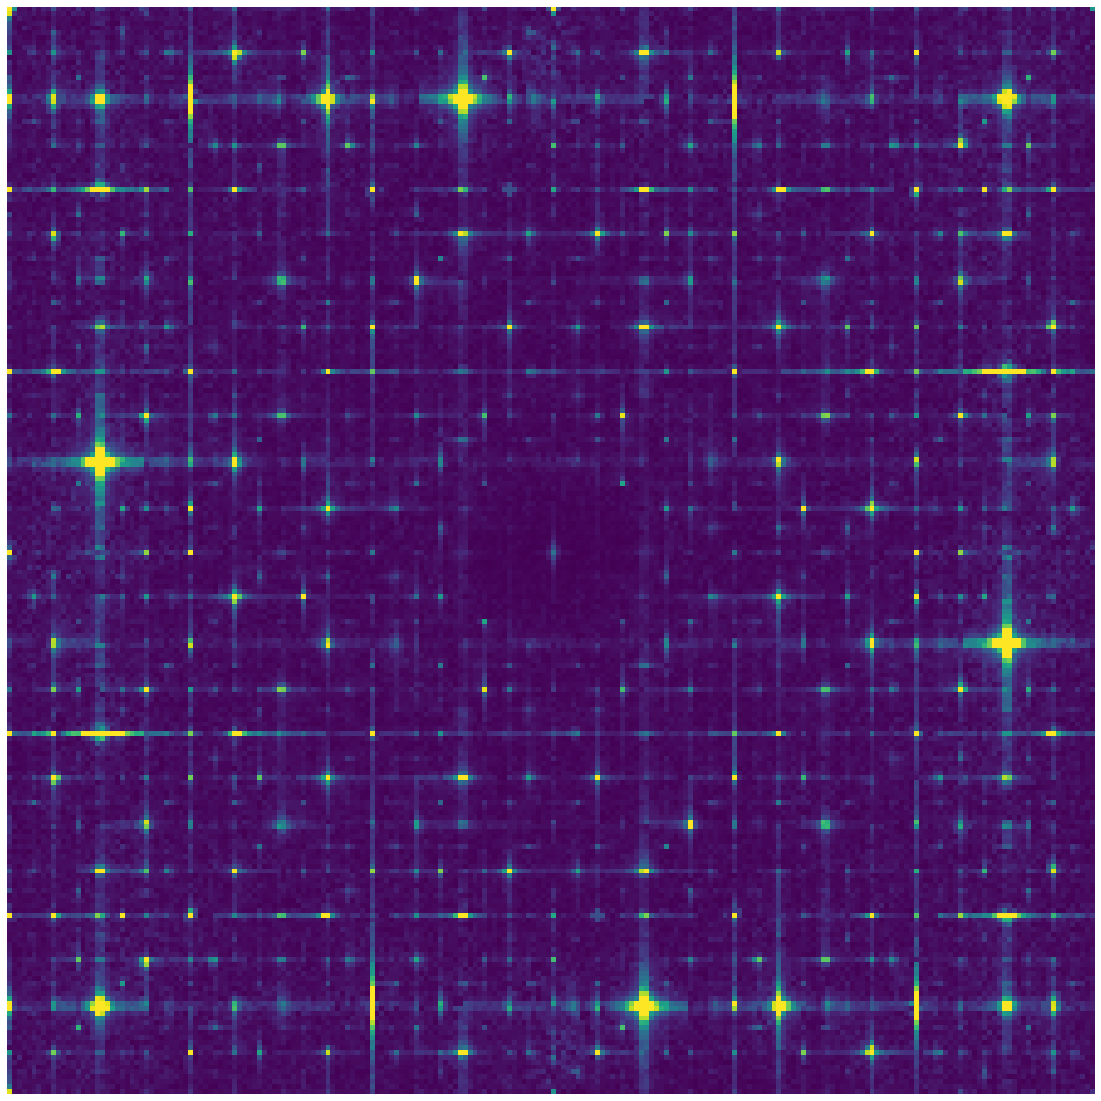
\includegraphics[width = 0.9 \textwidth]{figs/resfft_biggan.png}
      \caption{Big Gan}
    \end{minipage}
    \hfill
    \pause
		\begin{minipage}{0.3\textwidth}
      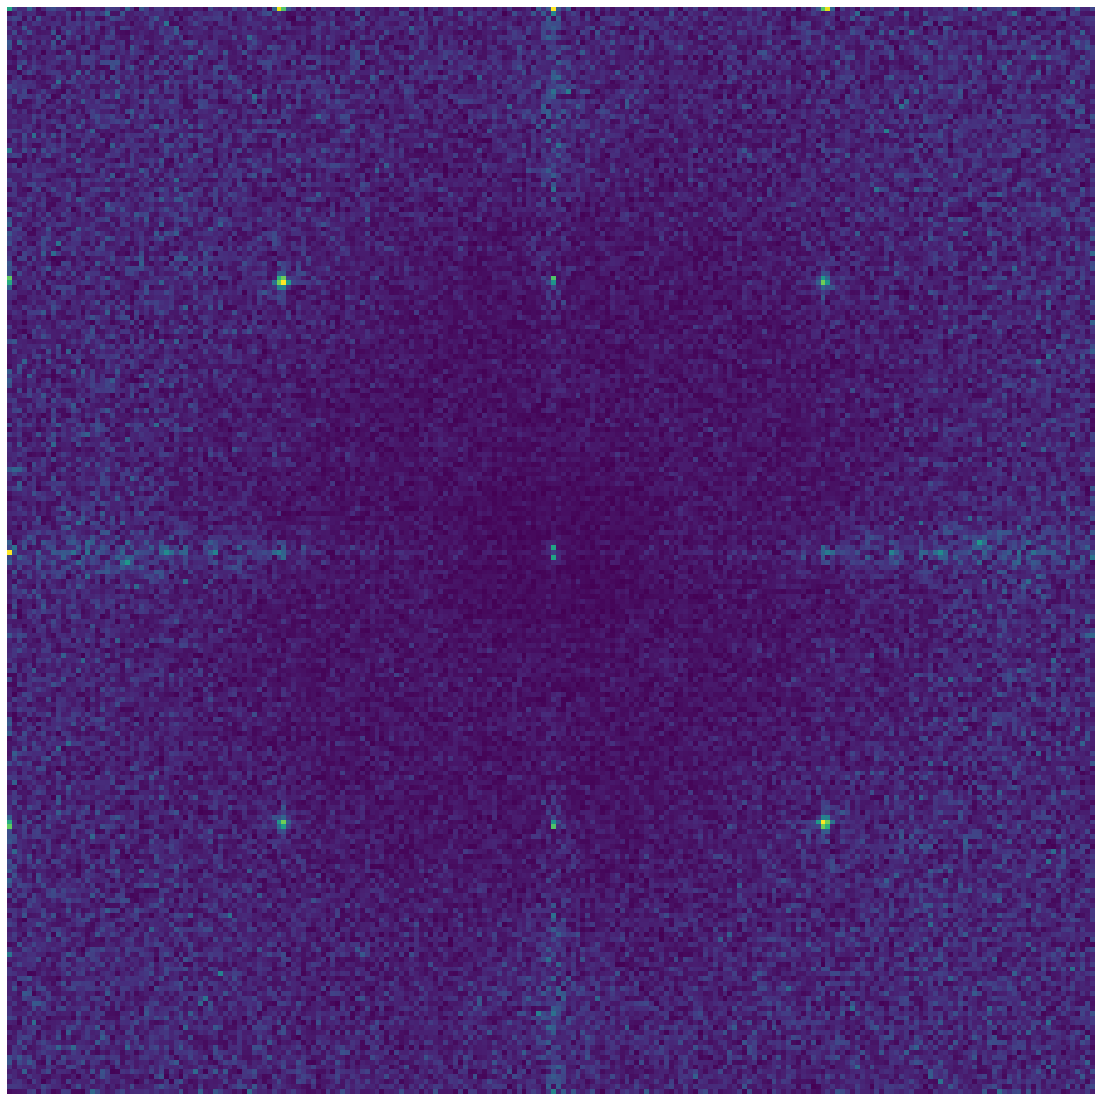
\includegraphics[width = 0.9 \textwidth]{figs/resfft_glide_text2img.png}
      \caption{Glide}
    \end{minipage}
    \hfill
    \pause
		\begin{minipage}{0.3\textwidth}
      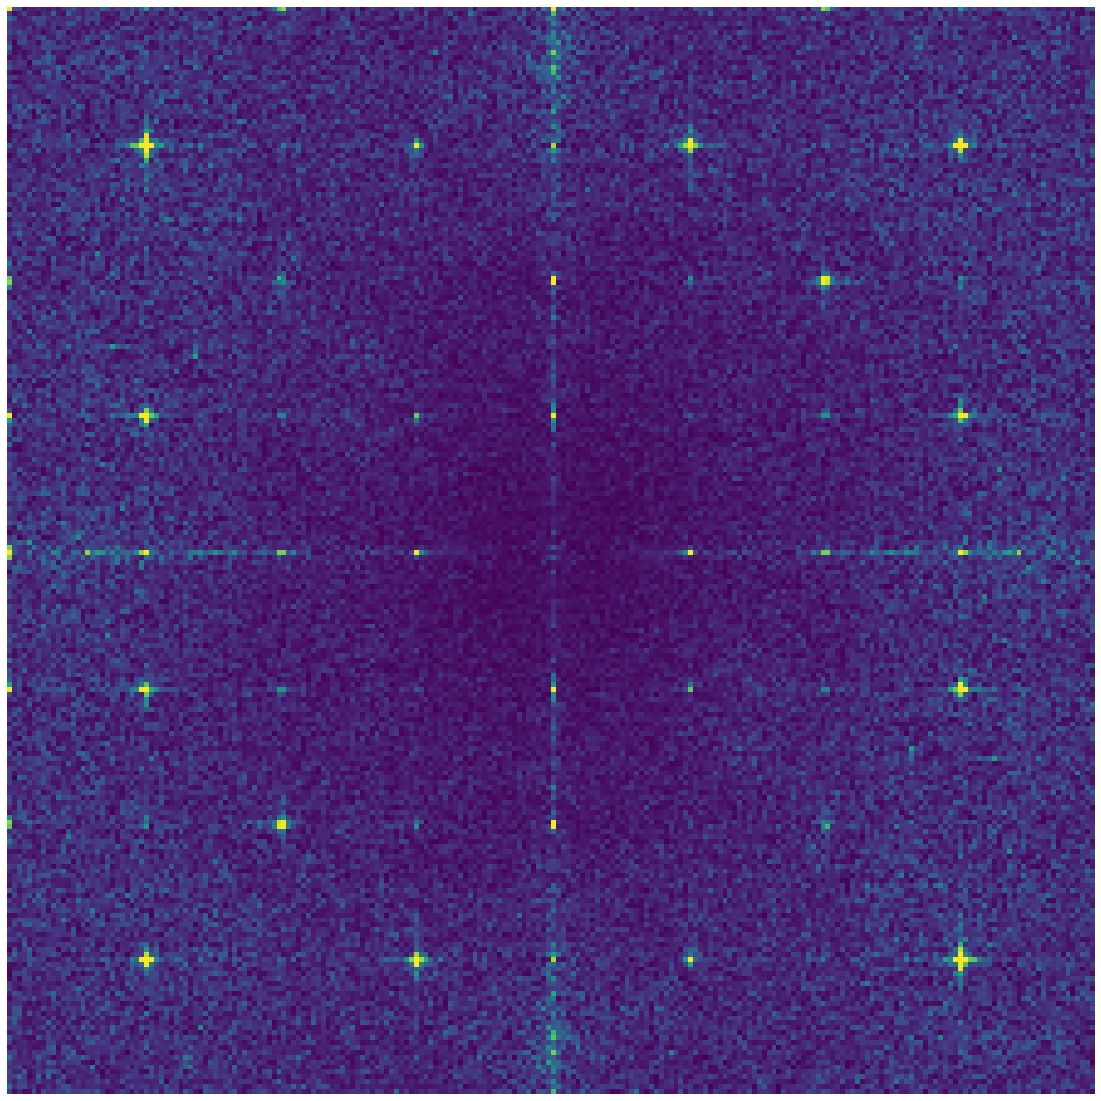
\includegraphics[width = 0.9 \textwidth]{figs/resfft_stable_diffusion.png}
      \caption{Stable Diffusion}
    \end{minipage}
	\end{figure}
  \text{\footnotesize source: Corvi et al, "ON THE DETECTION OF SYNTHETIC IMAGES GENERATED BY DIFFUSION MODELS", 2022}
\end{frame}

\begin{frame}
    \begin{minipage}{0.45\textwidth}
      GAN based
      \begin{itemize}
        \item NVIDIA GauGAN/Canvas
        \item Rosebud.AI
        \item DeepArt
        \item StyleGAN
        \item BigGAN
        \item ProGAN
        \item CycleGAN
        \item StarGAN
        \item Pix2Pix
        \item DiscoGAN
        \item WGAN-GP
      \end{itemize}
    \end{minipage}
		\begin{minipage}{0.45\textwidth}
      Diffusion based
      \begin{itemize}
        \item Stable Diffusion
        \item Midjourney
        \item DALL-E 3
        \item Adobe Firefly
        \item Runway Gen-2
        \item Google's Imagen/ImageFX
        \item Anthropic's Claude 3 Sonnet Vision
        \item Leonardo.AI
        \item ControlNet
        \item Kandinsky
        \item karlo-diffusion
      \end{itemize}
    \end{minipage}
\end{frame}

\section{Open Set Problem}
\begin{frame}
\begin{itemize}
    \item models shooting up left and right
    \item likely to encounter images from models not included in training
    \item classical approaches make oddly confident predictions since they cant express uncertainty
    \item approaches to solve this issue e.g. with multiple classifiers
\end{itemize}
\end{frame}

\section{Proposed Approach}
\begin{frame}
\begin{itemize}
    \item Bayesian Neural Networks
    \item key components, distribution over weights, updated according to bayes theorem
    \item measure uncertainty with variance of weights distribution, distribution over classes
    \item desired outcome with out-of-distribution data: low certainty
    \item desired outcome with post-processed images: robustness, or at least lost certainty with wrong predictions
\end{itemize}
\end{frame}

\begin{frame}
  \begin{figure}
    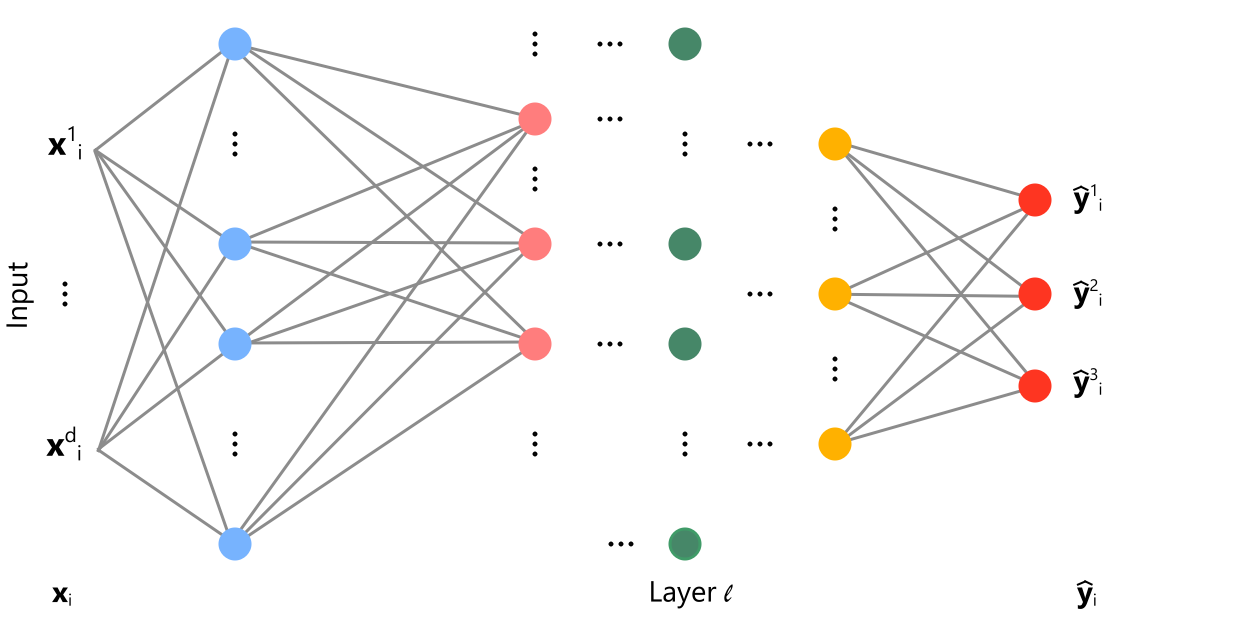
\includegraphics[width = 0.9 \textwidth]{figs/Ann.png}
  \end{figure}
  \text{\footnotesize source: Magris et al, "Bayesian Learning for Neural Networks: an algorithmic survey", 2022}
\end{frame}

\begin{frame}
  \begin{figure}
    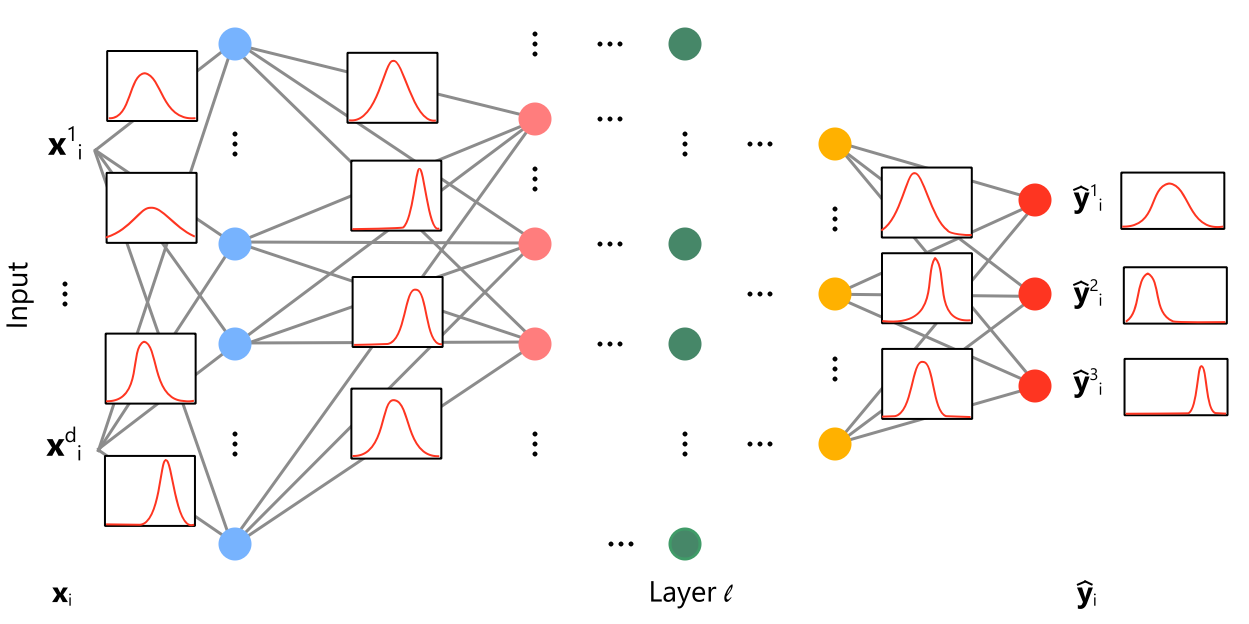
\includegraphics[width = 0.9 \textwidth]{figs/Bnn.png}
  \end{figure}
  \text{\footnotesize source: Magris et al, "Bayesian Learning for Neural Networks: an algorithmic survey", 2022}
\end{frame}

\begin{frame}
  Update model weights according to Bayes theorem
  \vfill
  \centering
  \begin{equation}
    P(w|D) = \frac{P(D|w) \cdot P(w)}{P(D)}
  \end{equation}
  \vfill
\end{frame}





\section{Timeline}
\begin{frame}
\begin{itemize}
    \item development of a baseline model with "classical" components
    \item development of a Bayesian Neural Network
    \item compare their predictive reliability
    \item compare performances on the open set problem
    \item compare the predictive reliability on post-processed images
    
\end{itemize}
\end{frame}

\end{document}
